%
% Carátula NO-oficial para 86.22 aboratorio de Control Automático.
%
% Basado en el template realizado por Diego Essaya, disponible en
%                                                         http://lug.fi.uba.ar
% Modificado por Patricio Moreno y Michel Peterson.
% Modificado por Sebastián Santisi.
% Abril 2014: Modificado por Patricio Moreno.
% Septiembre 2017: Modificado por Patricio Moreno.
% Septiembre 2017: Modificado por Ezequiel Pecker Marcosig.

%
% Acá se define el tamaño de letra principal:
% Para utilizar los estilos de KOMA-script, descomentar la línea siguiente y
% comentar la que le sigue (dejar sin comentar un único documentclass)
%\documentclass[10pt]{scrartcl}
\documentclass[10pt]{article}

%
% Título y autor(es):
%
\title{Trabajo Práctico N\b o 2}
\author{CERVETTO, Marcos\\MARCHI, Edgardo\\PECKER MARCOSIG, Ezequiel}

%------------------------- Carga de paquetes ---------------------------
%
% Si no necesitás algún paquete, comentalo.
%

%
% Definición del tamaño de página y los márgenes:
% Si preferís menos márgenes, descomentá la línea anterior
%\usepackage[a4paper,headheight=16pt,scale={0.7,0.8},hoffset=0.5cm]{geometry}

%
% Vamos a escribir en castellano:
%
\usepackage[spanish,es-tabla]{babel}
\usepackage[utf8x]{inputenc}

%
% Para escribir fórmulas matemáticas utilizamos:
%
\usepackage{amsmath}
\usepackage{amssymb}
%
% El paquete amsmath agrega algunas funcionalidades extra a las fórmulas.
% Además defino la numeración de las tablas y figuras al estilo "Figura 2.3",
% en lugar de "Figura 7". (Por lo tanto, aunque no uses fórmulas, si querés
% este tipo de numeración dejá el paquete amsmath descomentado).
%
% \numberwithin{equation}{section}
% \numberwithin{figure}{section}
% \numberwithin{table}{section}

%
% Para tener cabecera y pie de página con un estilo personalizado:
%
\usepackage{fancyhdr}

%
% Para poder controla mejor la poscición de las figuras
%
\usepackage{float}
\usepackage{placeins}
%
% Para poner el texto "Figura X" en negrita:
% (Si no tenés el paquete 'caption2', probá con 'caption').
%
\usepackage[hang,bf]{caption2}

%
% Para poner hipervínculos en el pdf
%
\usepackage[colorlinks=true,linkcolor=black, urlcolor=blue]{hyperref}

%
% Para poder modificar los items de las listas (IEEE style refs.)
%
\usepackage{enumerate}

%
% Para poder usar subfiguras: (al estilo Figura 2.3(b) )
%
%\usepackage{subfig}

%
% Para poder armar tablas con formato
%
\usepackage{booktabs}

%
% Para poder agregar notas al pie en tablas:
%
%\usepackage{threeparttable}

%------------------------------ graphicx ----------------------------------
%
% Para incluir imágenes, el siguiente código carga el paquete graphicx
% según se esté generando un archivo dvi o un pdf (con pdflatex).

% Para generar dvi, descomentá la linea siguiente:
%\usepackage[dvips]{graphicx}

% Para generar pdf, descomentá las dos lineas seguientes:
\usepackage[pdftex]{graphicx}
\pdfcompresslevel=9

%
% Todas las imágenes están en el directorio imgs:
%
\newcommand{\imgdir}{img}
\graphicspath{{\imgdir/}}

\usepackage{subfigure}
%
%------------------------------ graphicx ----------------------------------

% Necesitas este paquete si haces los diagrámas de flujo en el prográma Dia
% y exportás a latex
%\usepackage{tikz}

%------------------------------ color -------------------------------------
% Necesitas este paquete para definir tus propios colores
\usepackage{color}
\definecolor{mygreen}{rgb}{0,0.6,0}
\definecolor{mygray}{rgb}{0.5,0.5,0.5}
\definecolor{mymauve}{rgb}{0.58,0,0.82}
%------------------------------ color -------------------------------------


%----------------------------- listings -----------------------------------
% Necesitas este paquete para mostrar el código.
\usepackage{listings}
\lstset{
  breaklines=true,
  postbreak=\mbox{\textcolor{red}{$\hookrightarrow$}\space},
}
\lstdefinestyle{customcpp}{
  backgroundcolor=\color{white},   % choose the background color; you must add \usepackage{color} or \usepackage{xcolor}; should come as last argument
  basicstyle=\small,        % the size of the fonts that are used for the code
  breakatwhitespace=false,         % sets if automatic breaks should only happen at whitespace
  breaklines=true,                 % sets automatic line breaking
  captionpos=b,                    % sets the caption-position to bottom
  commentstyle=\color{mygreen},    % comment style
  deletekeywords={...},            % if you want to delete keywords from the given language
%  escapeinside={\%*}{*)},          % if you want to add LaTeX within your code
  extendedchars=true,              % lets you use non-ASCII characters; for 8-bits encodings only, does not work with UTF-8
  frame=single,	                   % adds a frame around the code
  keepspaces=true,                 % keeps spaces in text, useful for keeping indentation of code (possibly needs columns=flexible)
  keywordstyle=\color{blue},       % keyword style
  language=C++,                 % the language of the code
  morekeywords={*,...},           % if you want to add more keywords to the set
%  numbers=left,                    % where to put the line-numbers; possible values are (none, left, right)
%  numbersep=5pt,                   % how far the line-numbers are from the code
%  numberstyle=\tiny\color{mygray}, % the style that is used for the line-numbers
  rulecolor=\color{black},         % if not set, the frame-color may be changed on line-breaks within not-black text (e.g. comments (green here))
  showspaces=false,                % show spaces everywhere adding particular underscores; it overrides 'showstringspaces'
  showstringspaces=false,          % underline spaces within strings only
  showtabs=false,                  % show tabs within strings adding particular underscores
  stepnumber=2,                    % the step between two line-numbers. If it's 1, each line will be numbered
  stringstyle=\color{mymauve},     % string literal style
  tabsize=2,	                   % sets default tabsize to 2 spaces
  title=\lstname                   % show the filename of files included with \lstinputlisting; also try caption instead of title
}

\lstdefinestyle{custommatlab}{
  backgroundcolor=\color{white},   % choose the background color; you must add \usepackage{color} or \usepackage{xcolor}; should come as last argument
  basicstyle=\small,        % the size of the fonts that are used for the code
  breakatwhitespace=false,         % sets if automatic breaks should only happen at whitespace
  breaklines=true,                 % sets automatic line breaking
  captionpos=b,                    % sets the caption-position to bottom
  commentstyle=\color{mygreen},    % comment style
  deletekeywords={...},            % if you want to delete keywords from the given language
%  escapeinside={\%*}{*)},          % if you want to add LaTeX within your code
  extendedchars=true,              % lets you use non-ASCII characters; for 8-bits encodings only, does not work with UTF-8
  frame=single,	                   % adds a frame around the code
  keepspaces=true,                 % keeps spaces in text, useful for keeping indentation of code (possibly needs columns=flexible)
  keywordstyle=\color{blue},       % keyword style
  language=Matlab,                 % the language of the code
  morekeywords={*,...},           % if you want to add more keywords to the set
%  numbers=left,                    % where to put the line-numbers; possible values are (none, left, right)
%  numbersep=5pt,                   % how far the line-numbers are from the code
%  numberstyle=\tiny\color{mygray}, % the style that is used for the line-numbers
  rulecolor=\color{black},         % if not set, the frame-color may be changed on line-breaks within not-black text (e.g. comments (green here))
  showspaces=false,                % show spaces everywhere adding particular underscores; it overrides 'showstringspaces'
  showstringspaces=false,          % underline spaces within strings only
  showtabs=false,                  % show tabs within strings adding particular underscores
  stepnumber=2,                    % the step between two line-numbers. If it's 1, each line will be numbered
  stringstyle=\color{mymauve},     % string literal style
  tabsize=2,	                   % sets default tabsize to 2 spaces
  title=\lstname                   % show the filename of files included with \lstinputlisting; also try caption instead of title
}
%----------------------------- listings -----------------------------------



%------------------------- Inicio del documento ---------------------------

\begin{document}

%
% Hago que en la cabecera de página se muestre a la derecha la sección,
% y en el pie, en número de página a la derecha:
%
\pagestyle{fancy}
\lhead{\sc TP Nº2 - \sc 2º Cuat. 2017}
\chead{}
\rhead{CERVETTO, MARCHI, PECKER MARCOSIG}
\lfoot{}
\cfoot{}
\rfoot{\thepage}

%
% Carátula:
%
\begin{titlepage}

\thispagestyle{empty}

\begin{center}
%
\includegraphics[scale=0.3]{img/fiuba}\\

\includegraphics[scale=0.7]{img/fcenuba}\\
\large{\textsc{Universidad de Buenos Aires}}\\
\large{\textsc{Facultad De Ciencias Exactas y Naturales}}\\
\large{\textsc{Departamento de Computación}}\\
% Modificar año y cuatrimestre
\small{Año 2017 - 2\textsuperscript{do} Cuatrimestre}
\end{center}

\vfill

\begin{center} % Modificar el código de ser necesario
\Large{\underline{\textsc{Simulación de Eventos Discretos}}}
\end{center}

\vfill

\begin{tabbing}
\hspace{2cm}\=\+TRABAJO PRÁCTICO Nº \textless{}2\textgreater{}\\
	TEMA:\textless{}Manejo del Inventario de una Industria\textgreater{}\\
	FECHA:\textless{\today}\textgreater{}\\
\\
	INTEGRANTES:\hspace{-1cm}\=\+\hspace{1cm}\=\hspace{6cm}\=\\
		CERVETTO, Marcos	\>\>- \#FIUBA\\
			\>\footnotesize{\verb!<cervettomarcos@gmail.com>!}\\
		MARCHI, Edgardo	\>\>- \#FIUBA\\
			\>\footnotesize{\verb!<edgardo.marchi@gmail.com>!}\\
		PECKER MARCOSIG, Ezequiel	\>\>- \#FIUBA\\
			\>\footnotesize{\verb!<ezepecker@gmail.com>!}\\
\end{tabbing}

\vfill

\hrule
\vspace{0.2cm}

% Modificar código de ser necesario
\noindent\small{Simulación de Eventos Discretos}

\end{titlepage}

%
% Hago que las páginas se comiencen a contar a partir de aquí:
%
\setcounter{page}{1}

%
% Pongo el índice en una página aparte:
%
\tableofcontents
\newpage

%
% Inicio del TP:
%

\section{Objetivo y Enunciado}
%El objetivo de este Trabajo Práctico es demostrar la comprensión del modelado y simulación utilizando el formalismo DEVS, junto a la aplicación de las técnicas mediante la herramienta CD++.
%Se deberá identificar un sistema del mundo real que pueda ser representado usando DEVS y construir luego un modelo del mismo.
%Finalmente se ejecutarán simulaciones del sistema analizado. El sistema estudiado puede ser natural o artificial, y puede existir en la realidad o no.

\section{Modelo Conceptual}
\subsection{Motivación\label{sec:motivacion}}

Una compañía que vende un único producto está interesada en estudiar la forma óptima de ordenamiento de las unidades producidas en el almacén.

En la Figura \ref{fig:esquema-del-problema} se muestra un esquema de la industria, donde se observa la ubicación del inventario.

Para este trabajo, el bloque Inventario se va a modelizar con autómata celular.

\begin{figure}[h]
\centering
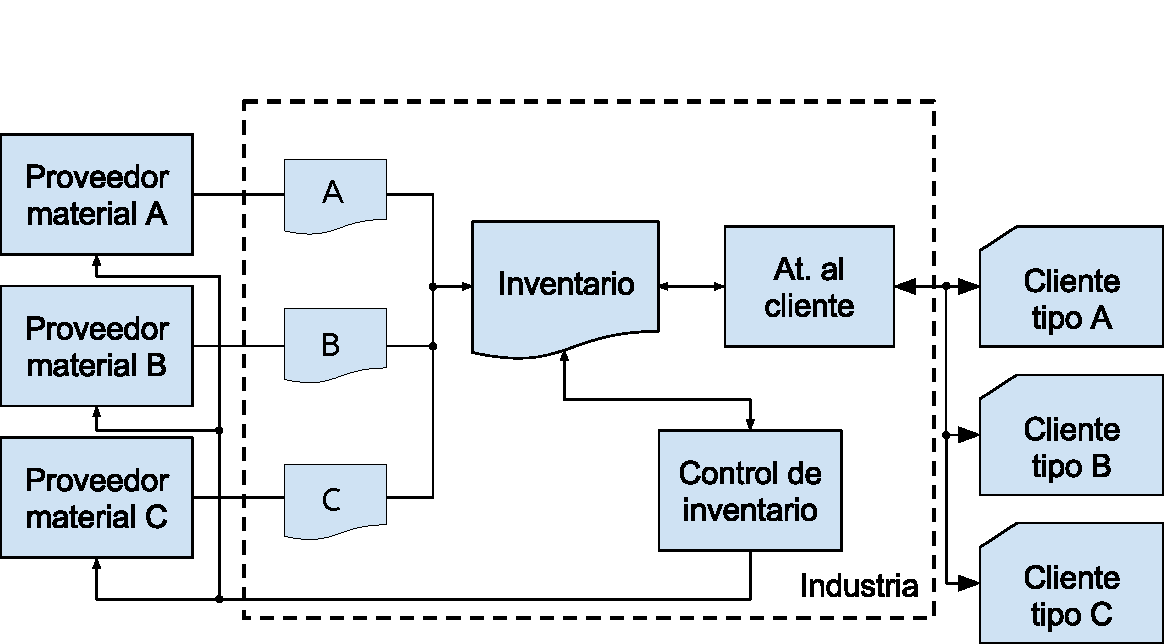
\includegraphics[width=\textwidth]{img/figura1}
\caption{Esquema del problema planteado.}
\label{fig:esquema-del-problema}
\end{figure}
\FloatBarrier 

\subsection{Autómata Celular\label{sec:AC}} 

 El bloque atómico DEVS correspondiente al Inventario que se indica en la Figura \ref{fig:esquema-del-problema} va a ser reemplazado por tres bloques cell-DEVS, según la Figura \ref{fig:AC-esquematico}.
 
 \begin{figure}[h] 
 	\centering
 	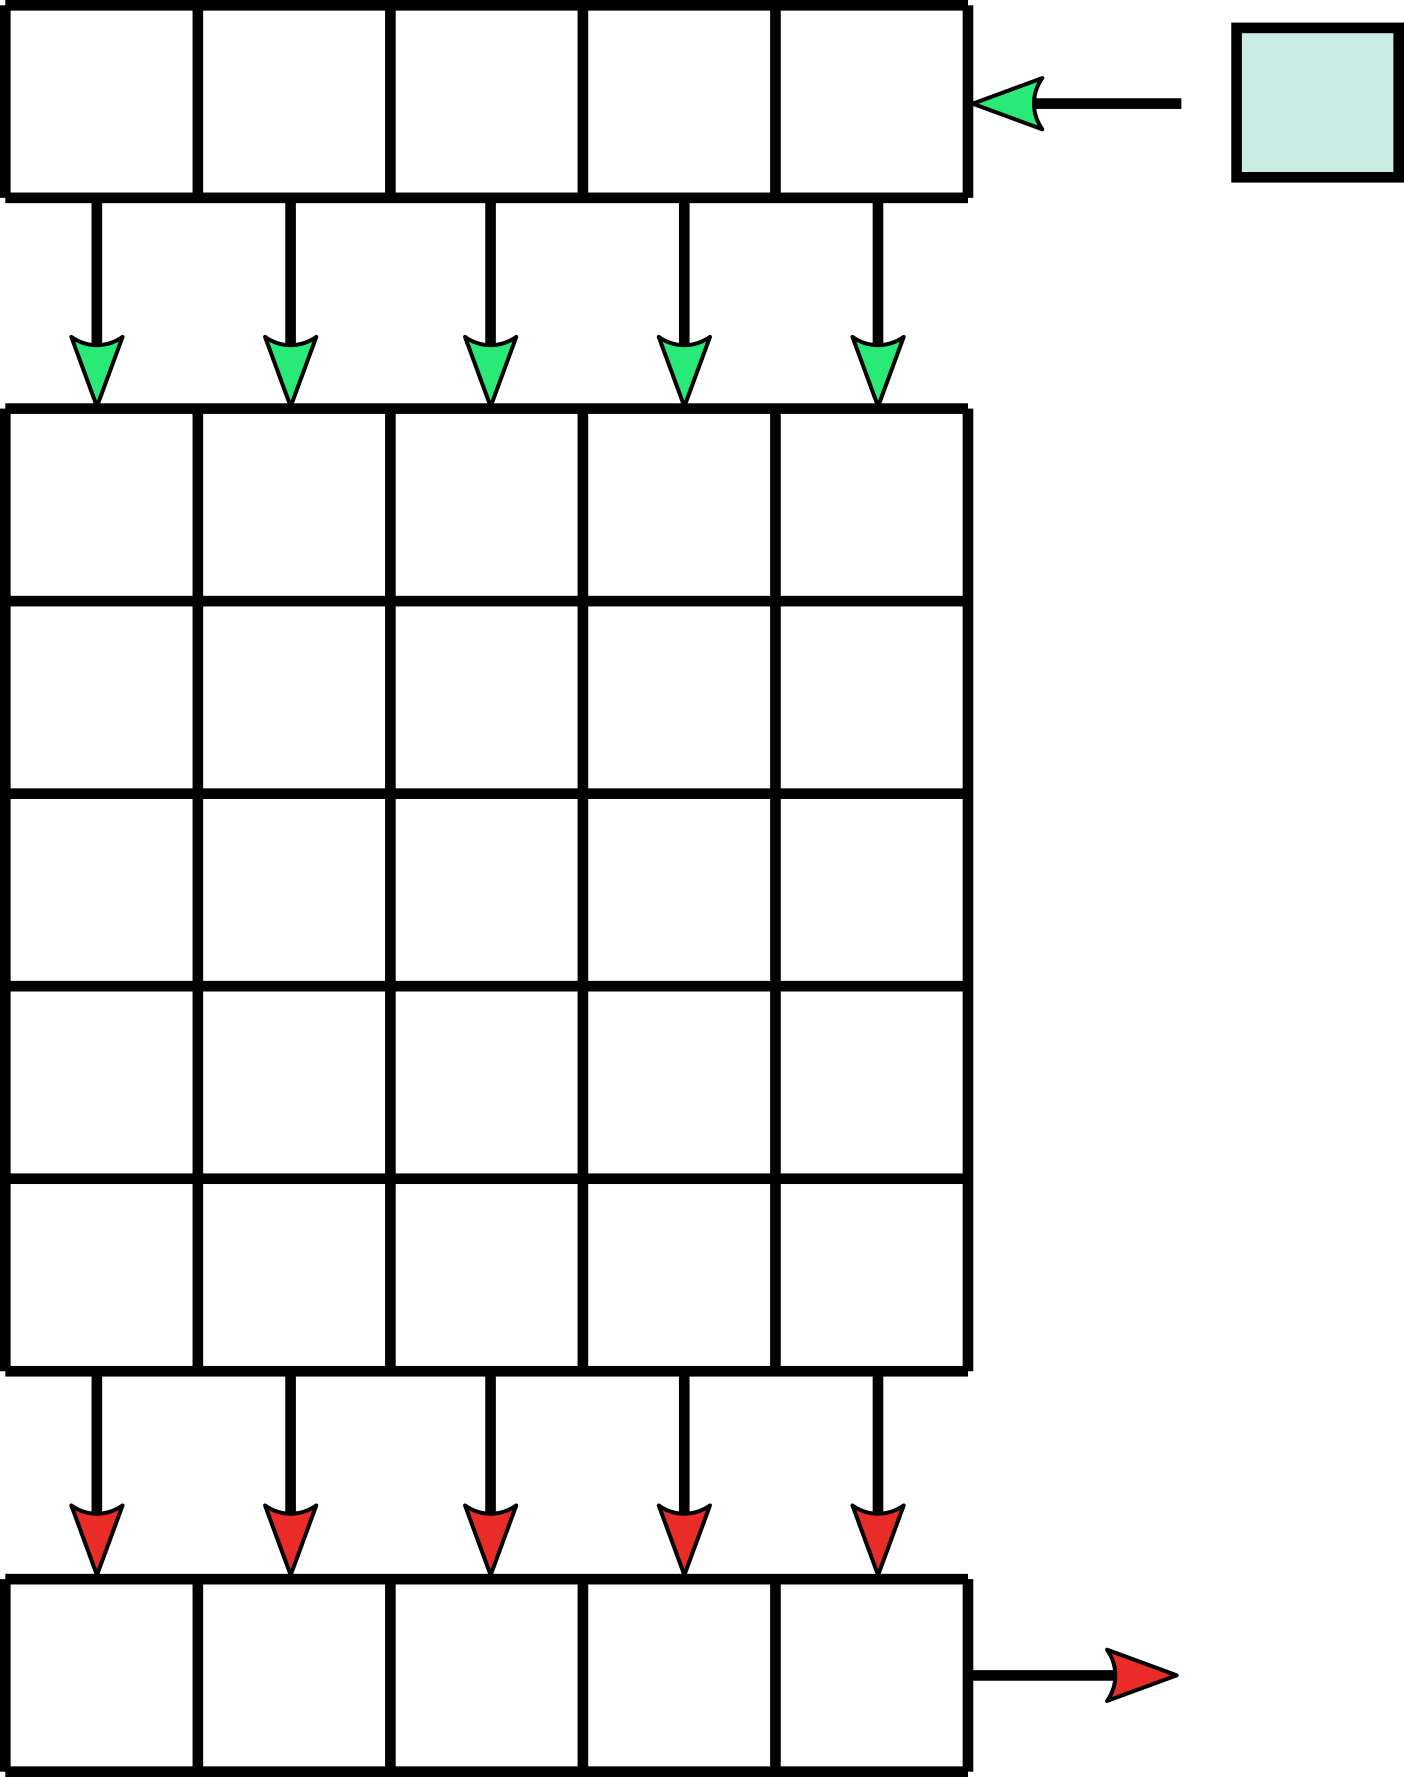
\includegraphics[width=0.5\textwidth]{grilla} 
 	\caption{Inventario con cell-DEVS.} 
 	\label{fig:AC-esquematico} 
 \end{figure}
 \FloatBarrier
 
 El primer bloque corresponde a una fila de celdas que manejarán la ubicación inicial de los productos dentro del inventario. Del trabajo 1 se puede recordar que cada producto tiene una fecha de vencimiento asociada. Esta fecha será la que determine la columna en la que se apilará a cada producto. Por ejemplo: si falta menos de una semana para su vencimiento se apilará en la columna 0 (más a la derecha), si falta entre 1 y 2 semanas en la columna 1, entre 2 y 3 en la columna 2, etc. Este proceso se esquematiza en la Figura \ref{fig:AC-ingreso-de-productos}.
 
 \begin{figure}[h] 
 	\centering 
 	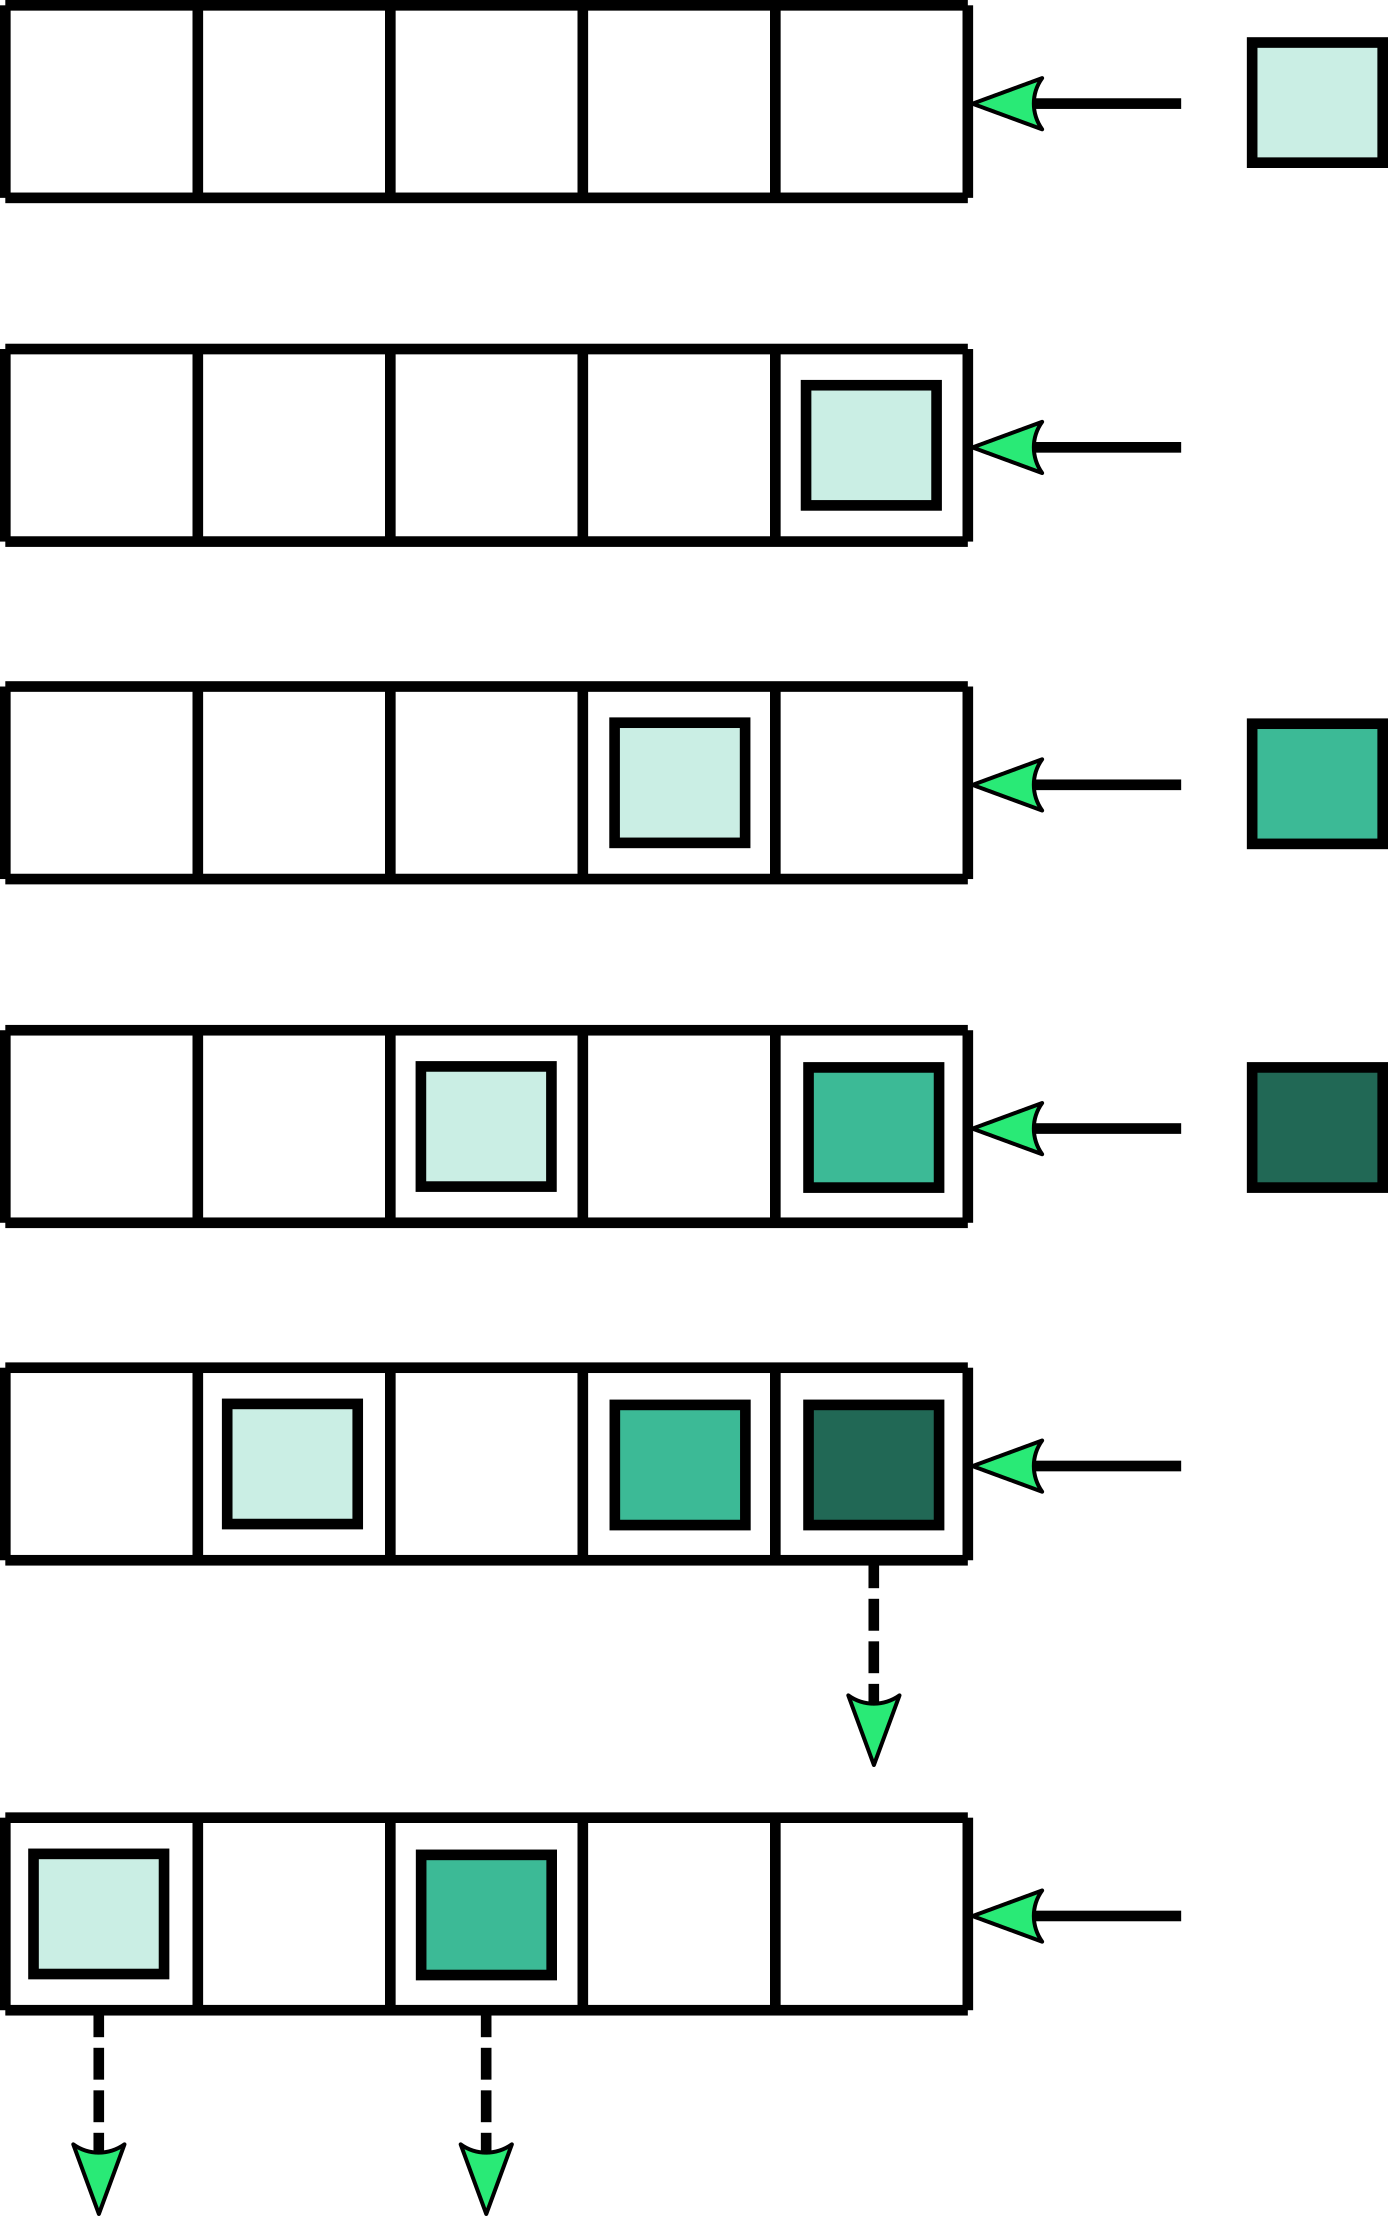
\includegraphics[width=0.5\textwidth]{entrada} 
 	\caption{Ingreso de productos al inventario.} 
 	\label{fig:AC-ingreso-de-productos} 
 \end{figure}
 \FloatBarrier
 
 El segundo bloque será el inventario propiamente dicho. Es una grilla donde las columnas representan posiciones de apilamiento de productos. Las entradas de productos se realizan por la parte superior de cada columna, de forma de ir apilándolos. La salida de productos se realiza por la parte inferior de cada columna. Periódicamente se chequea la fecha de vencimiento de cada producto, y si cumple la condición de la columna siguiente a la derecha, por ejemplo que falte menos de N semanas para que perezca, el producto se intenta mover a esa columna.
 
 La salida de productos está físicamente cercana a la columna derecha (la que contiene a los productos más próximos a vencer). El encargado de retirar productos demora un tiempo hasta llegar a la columna N por lo que idealmente se prefiere retirar los productos de la columna 0. Sin embargo si no hay productos con una fecha de vencimiento tan próxima, deberá recorrer las columnas hasta llegar a un producto. Este proceso de retiro de elementos se modela con el tercer bloque cell-DEVS, en este caso también de una sola fila.
 Todo este proceso se puede observar en la figura en la Figura \ref{fig:AC-inventario}. La fecha de vencimiento se grafica según el esquema de colores de la Figura \ref{fig:AC-colores}.
 
 \begin{figure}[h] 
 	\centering 
 	
\includegraphics[width=0.3\textwidth]{colores} 
 	\caption{Codificación de colores por fecha de vencimiento.} 
 	\label{fig:AC-colores} 
 \end{figure}
 
 \begin{figure}[h] 
 \centering
 
 	\begin{tabular}{cc}
 		\multicolumn{2}{c}{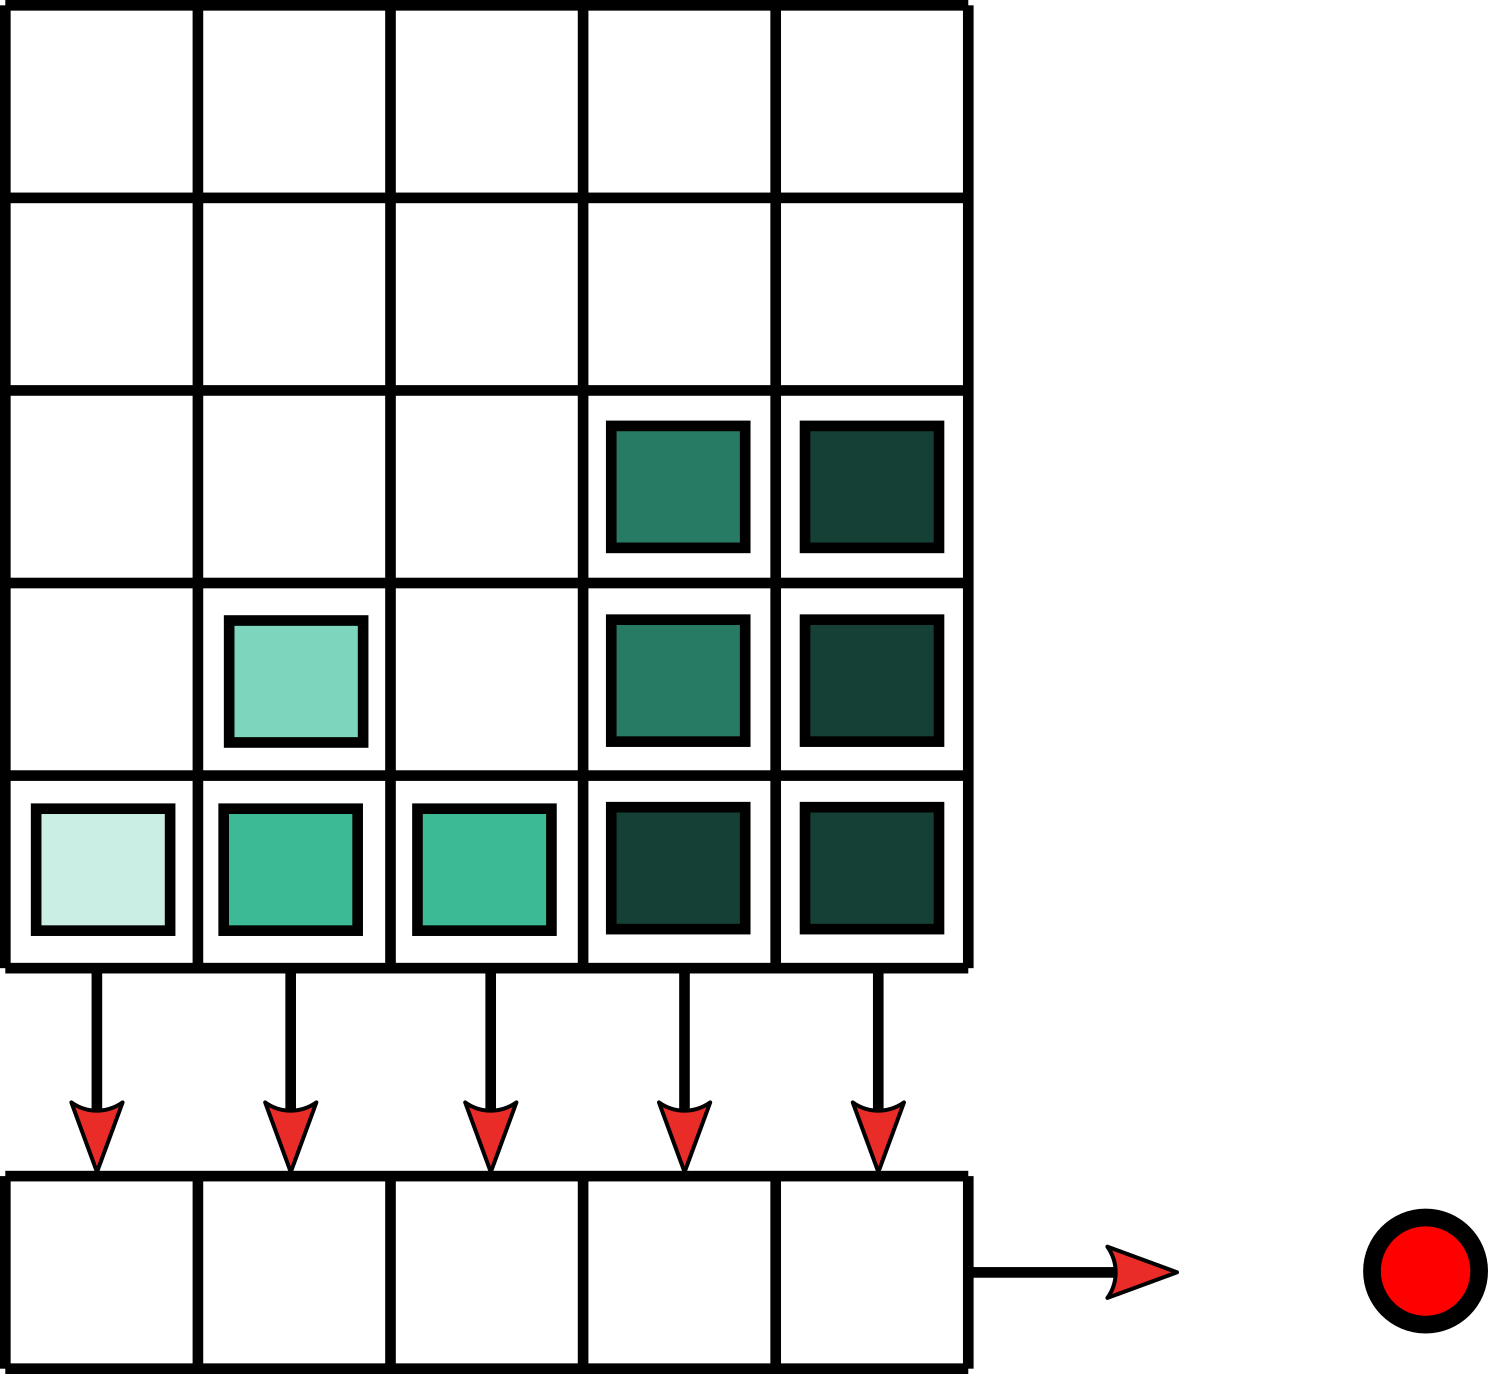
\includegraphics[width=0.4\linewidth]{pedido1}}\\[5mm]
 		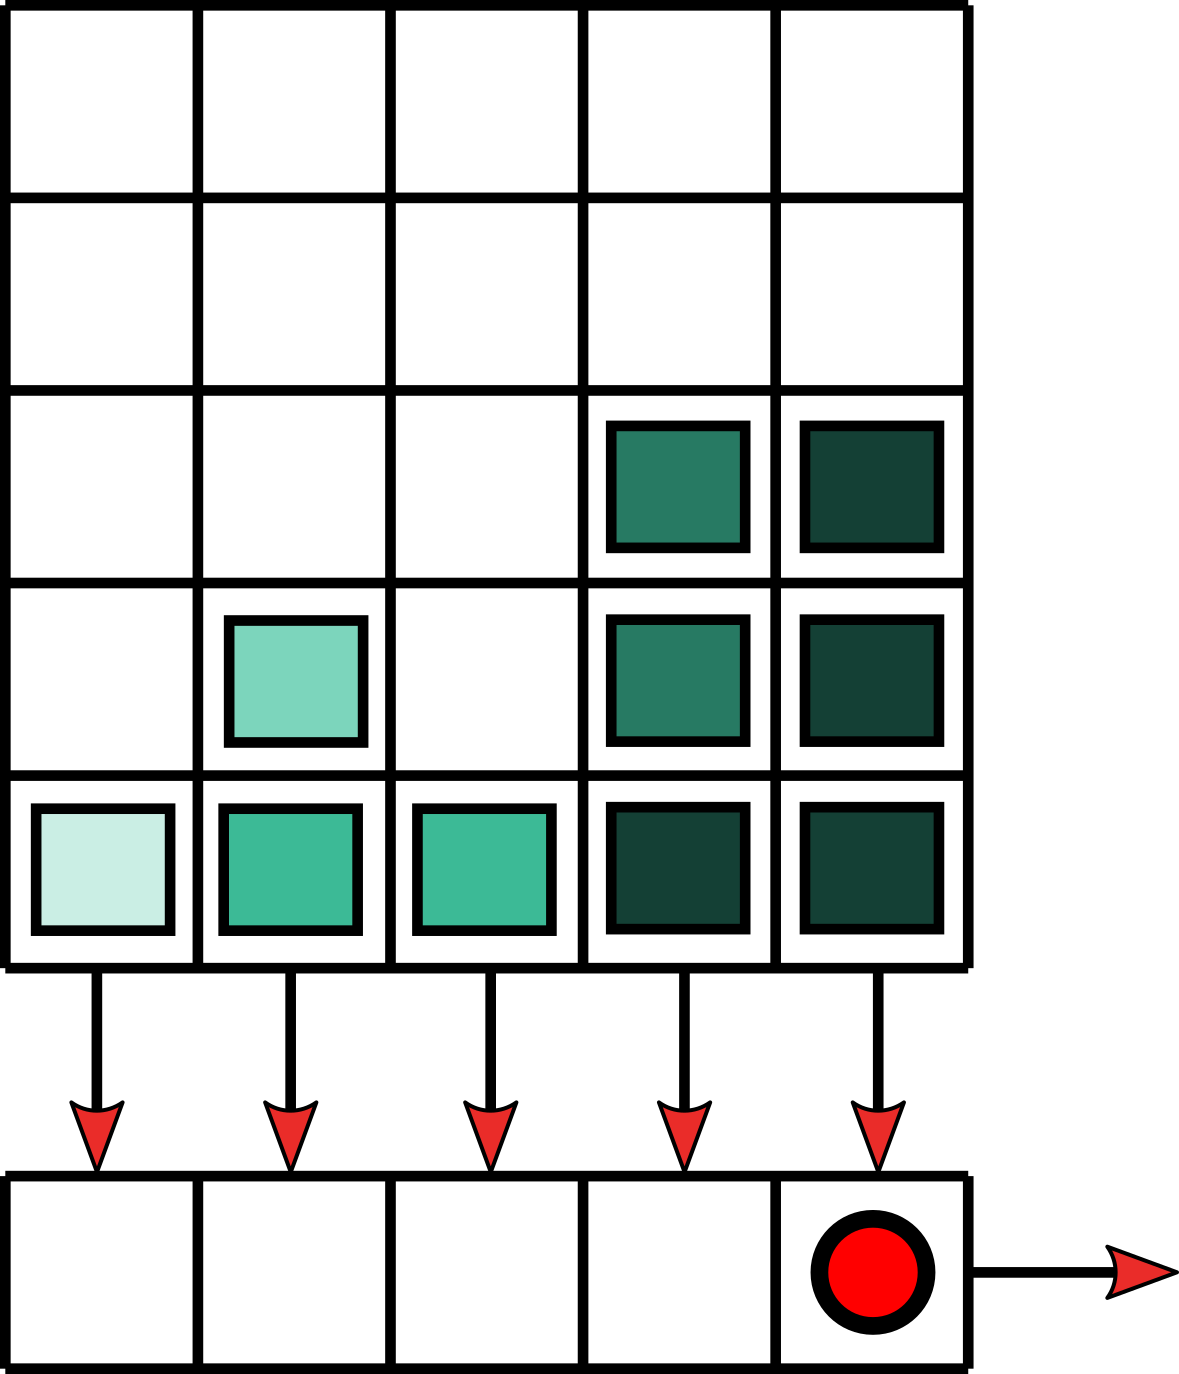
\includegraphics[width=0.3\linewidth]{pedido2} &
 		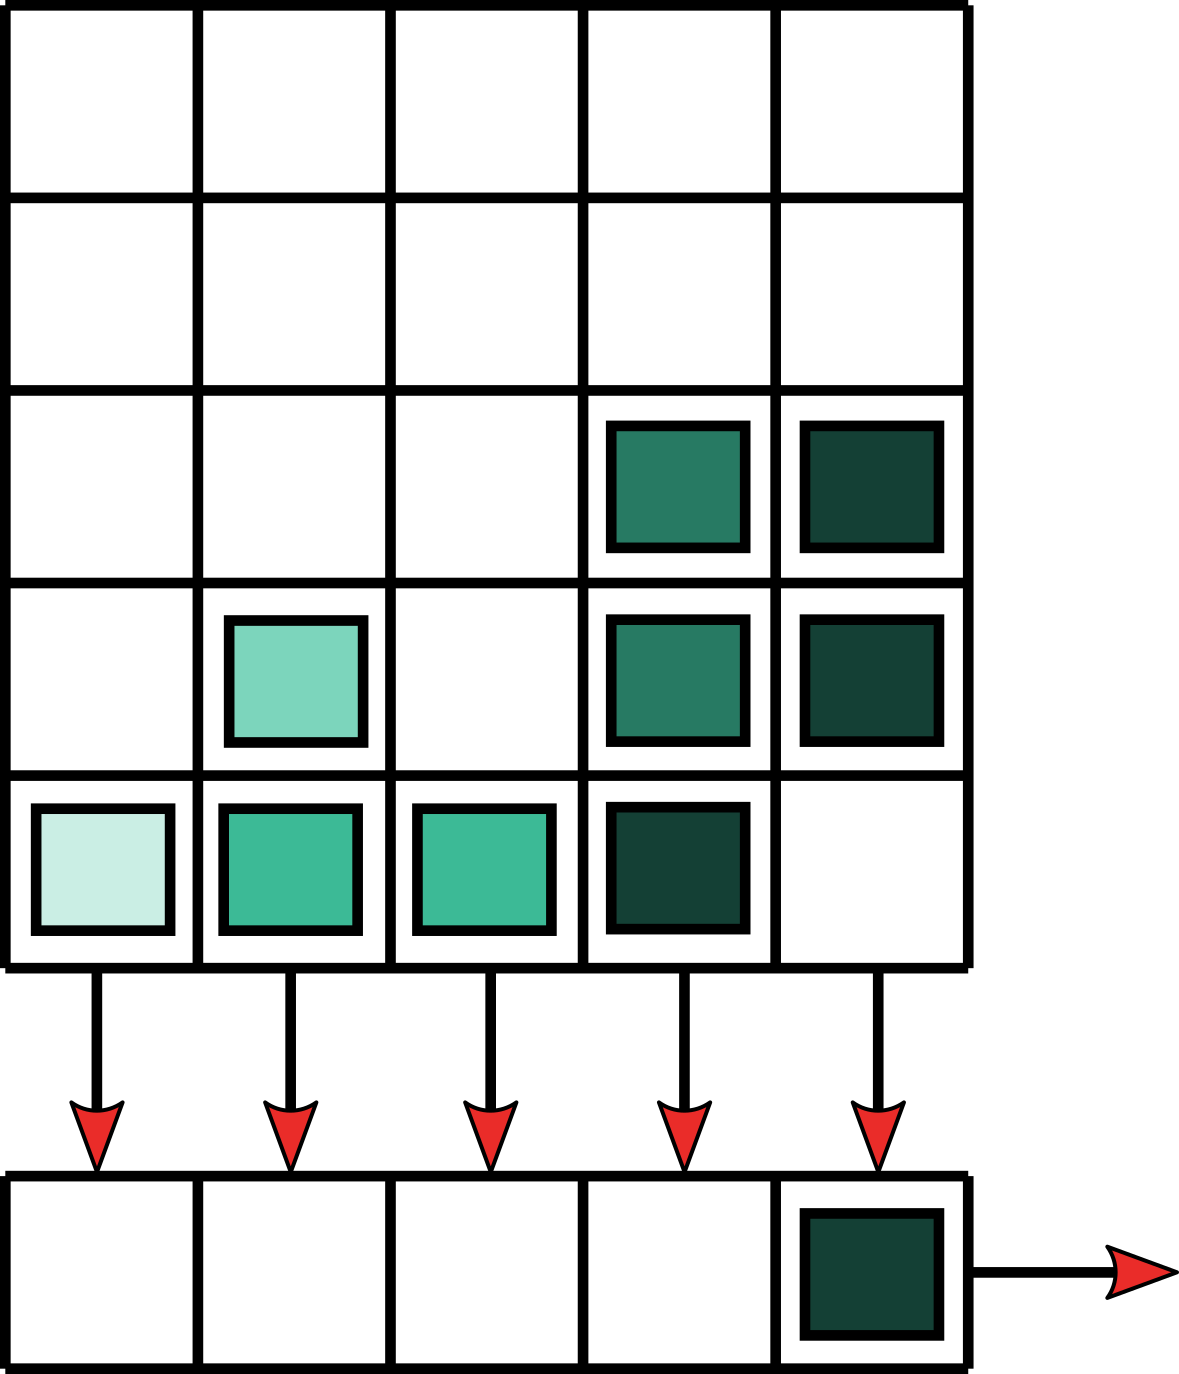
\includegraphics[width=0.3\linewidth]{pedido3} \\[5mm]
 		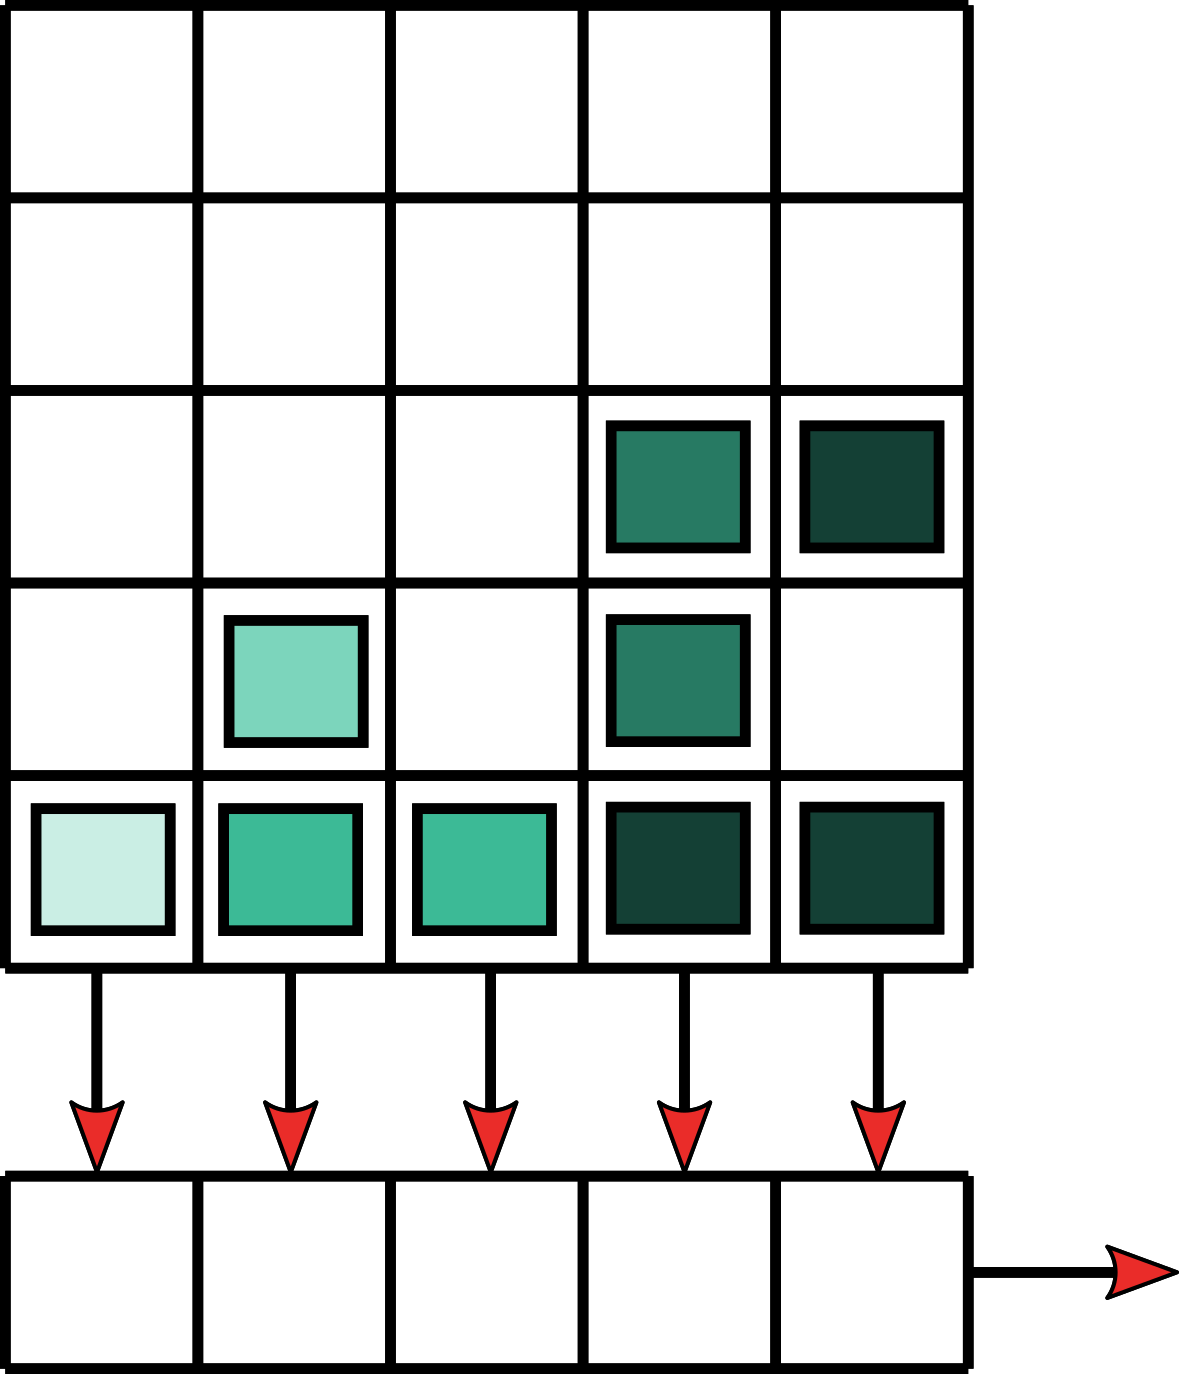
\includegraphics[width=0.3\linewidth]{pedido4} &
 		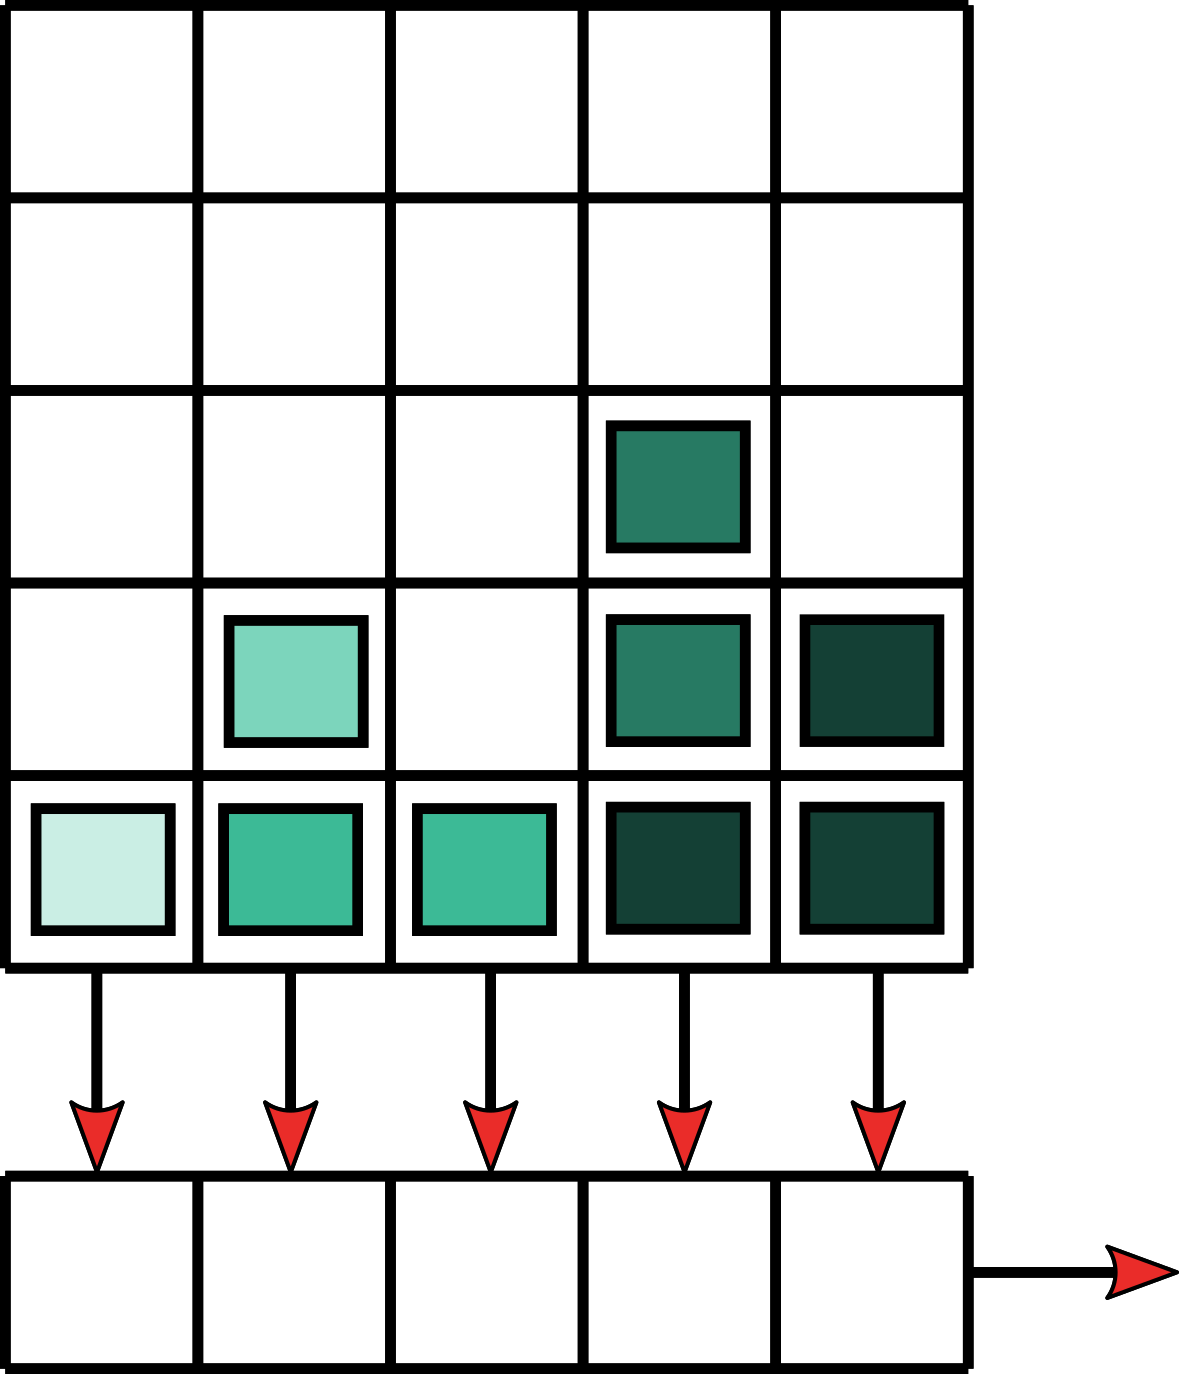
\includegraphics[width=0.3\linewidth]{pedido5} \\
 	\end{tabular}
 	
 	\caption{Autómata celular del inventario.} 
 	\label{fig:AC-inventario} 
 \end{figure}
 \FloatBarrier
 
\subsection{Celdas}

El objetivo del autómata celular es ordenar los productos en el almacén de modo que aquellos con fecha de vencimiento más próxima queden ubicados espacialmente más cerca de la salida, de modo de ser despachados más rápido. De esta manera se busca reducir la cantidad de productos vencidos dentro del almacén. Para esto, periódicamente se revisan las fechas de vencimiento de los productos estampadas en un código de barras en cada unidad. Su ubicación depende del valor de su fecha de vencimiento. Los productos sólo pueden ser movidos si la columna adyacente a la derecha tiene una ubicación disponible hasta un nivel por encima de la altura de ubicación del producto.
Cabe destacar que si la ubicación inferior a donde se encuentra un producto está libre, el producto baja hasta estar apoyado sobre otro producto o sobre el suelo del depósito.
Por estos motivos (y por la preferencia de movimiento hacia la derecha) el vecindario propuesto se puede ver en la Figura~\ref{fig:AC-vecindario}.

\begin{figure}[h] 
  \centering 
  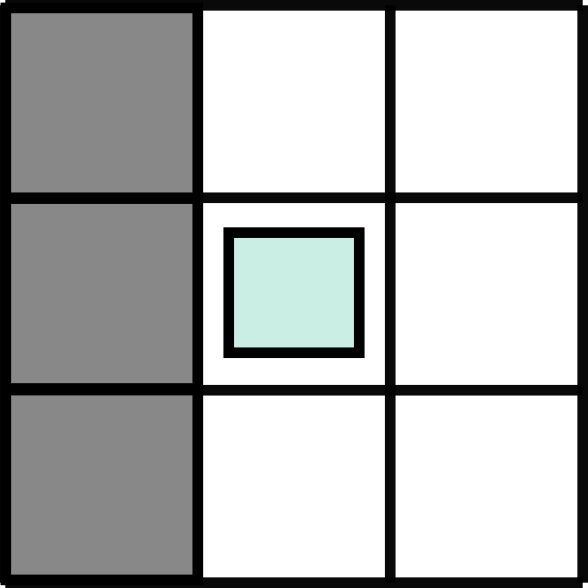
\includegraphics[width=0.3\textwidth]{vecindario} 
  \caption{Vecindario.} 
  \label{fig:AC-vecindario} 
\end{figure}
\FloatBarrier

Las preguntas a responder mediante simulaciones son:
\begin{itemize}
\item \textit{¿Qué política de ordenamiento permite reducir la cantidad de unidades vencidas al momento del despacho?}
\item Y conectada con la pregunta anterior, \textit{¿qué política de ordenamiento permite disminuir el tiempo necesario para despachar una unidad?}
\end{itemize}
% \FloatBarrier

\section{Descripción Formal}

\subsection{\textit{Top-Model}}

\subsection{Cinta Transportadora}\label{sec:CT}

La cinta transportadora es el dispositivo por el que ingresan los productos al inventario. La cinta tiene su entrada \texttt{in} por la derecha en la celda $(0,n)$. Además cada celda tiene asociadas una entrada \texttt{ini} y una salida \texttt{outi}, como se observa en la Figura~\ref{fig:CT-automata}. 

\begin{figure}[h] 
  \centering 
  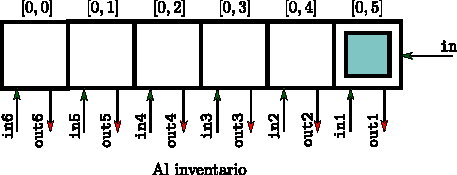
\includegraphics[width=0.8\textwidth]{CT-automata.pdf} 
  \caption{Autómata celular de la cinta transportadora.} 
  \label{fig:CT-automata} 
\end{figure}
\FloatBarrier


Los productos ingresan por la entrada \texttt{in} y se van desplazando hacia la izquierda a una velocidad representada por el tiempo entre ejecuciones de las reglas.

Para cada celda en este autómata celular importa solamente el valor de la celda anterior y el de la celda posterior. Por este motivo el vecindario está definido en la Figura~\ref{fig:CT-vecindario}.

\begin{figure}[h] 
  \centering 
  
\includegraphics[width=0.4\textwidth]{CT-vecindario.pdf} 
  \caption{Vecindario de la cinta transportadora.} 
  \label{fig:CT-vecindario} 
\end{figure}
\FloatBarrier

Cada elemento de la cinta transportadora está asociado a una columna en el inventario. A su vez, cada columna en el inventario tiene asignado un rango de fechas de vencimiento posibles, estando más hacia la izquierda las columnas asociadas a vencimientos más remotos.

Las consultas de lugar disponible en una columna del inventario se realizan enviando un valor de fecha de vencimiento imposible, en este caso igual a $-1$. El inventario debe responder con $0$ si no hay lugar en la columna por la que se consultó o un número no nulo en caso contrario. En caso que la respuesta del inventario sea que no hay lugar en la columna por la que se consultó entonces la cinta debe hacer avanzar al producto hacia la izquierda una posición más y volver a preguntar por la disponibilidad de espacio en el inventario.

Cada elemento en la cinta transportadora se representa con una tupla de tres elementos: \texttt{[ID columna, producto, indicador]}. El \texttt{ID columna} representa el rango de fechas de vencimiento asociados a la celda y a la columna respectiva del inventario. El elemento \texttt{producto} lleva la fecha de vencimiento del producto. Por último, el elemento \texttt{indicador} puede tener distintos significados dependiendo de su valor, los valores que puede tomar son: $0$, $1$ ó $2$. Si vale $1$ significa que el producto está listo para ser ubicado en la columna del inventario asociada a la celda actual de la cinta transportadora pero que no había lugar, si en cambio vale $2$ significa que ninguna de las columnas del inventario por las que se consultó tenía espacio y entonces ese producto permanecerá en la cinta transportadora.

Los elementos de las tuplas se acceden utilizando el signo de exclamación e indicando a continuación el elemento que se quiere acceder. Así por ejemplo el elemento $0$ o \texttt{ID} de la celda actual se accede mediante $(0,0)!0$.

Las reglas tienen la siguiente sintaxis: 
\begin{lstlisting}
rule : { resultado } { demora } { condicion }}
\end{lstlisting}

Las reglas que representan a la descripción anterior y están asociadas a las células de este autómata celular se enumeran a continuación:

\begin{minipage}{1\textwidth}
	\centering
	\begin{lstlisting}
[cinta-reglas]
rule : { [(0,0)!0,(0,1)!1,0] } { 100 } { NOT isUndefined((0,1)!1) AND (0,1)!1 != 0 AND (0,1)!1 > (0,1)!0 + time/1000 }
rule : { [(0,0)!0,0,0] } { 100 } { NOT isUndefined((0,-1)!1) AND (0,0)!1 != 0 AND (0,0)!1 > (0,0)!0 + time/1000 AND (0,-1)!1 = 0 } 
rule : { [(0,0)!0,(0,1)!1,0] } { 100 } { (0,1)!2 = 1 }
rule : { [(0,0)!0,0,0] } { 100 } { (0,0)!2 = 1 AND NOT isUndefined((0,-1)!1) AND (0,-1)!1 = 0 }
rule : { [(0,0)!0,(0,0)!1,2] } { 100 } { (0,0)!2 = 1 AND (isUndefined((0,-1)!1) OR (0,-1)!1 != 0) }
rule : { [(0,0)!0,(0,0)!1+send(output,-1),0] } { 100 } { (0,0)!2 != 2 AND (0,0)!1 != 0 AND (0,0)!1 <= (0,0)!0 + time/1000 }
rule : { (0,0) } 0 { t }
	\end{lstlisting}
\end{minipage}

La primera regla pregunta si la celda que está a la derecha de la celda actual está definida (\texttt{NOT isUndefined((0,1)!1)}), tiene un producto (\texttt{(0,1)!1 != 0}) y la fecha de vencimiento del producto es mayor que la de la columna (\texttt{(0,1)!1 > (0,1)!0 + time/1000}). En caso que se cumpla se mueve el producto desde la celda de la derecha a la celda actual.

La segunda regla es el complemento de la primera, es decir, pregunta si la celda de la izquierda está definida (\texttt{NOT isUndefined((0,-1)!1)}) y está vacía (\texttt{(0,-1)!1 = 0}) y en la celda actual hay un producto y su fecha de vencimiento es mayor que la de la columna (\texttt{(0,0)!1>(0,0)!0+time/1000}). Si se cumple, entonces se quita el producto de esta celda.

La tercera regla verifica si el elemento \texttt{indicador} de la tupla de la celda de la derecha es $1$. Si es así significa que la cinta consultó al inventario para mover ese producto y éste le respondió que no había lugar. Entonces lo que se hace es mover ese producto a la siguiente celda hacia la izquierda.

La cuarta regla es el complemento de la tercera regla, pues pregunta si el elemento \texttt{indicador} de la tupla de la celda actual es $1$ y si la celda de la izquierda está vacía. Si se cumple entonces quita al producto de esta celda.

La quinta regla se ejecuta cuando el producto no puede ser descargado en el inventario porque no hay lugar en las columnas que pregunta y alcanza el extremo izquierdo de la cinta transportadora. Esta condición se indica escribiendo un $2$ en el elemento indicador de la celda.

La sexta regla es la que permite hacer la consulta al inventario de si hay lugar en la columna correspondiente. Esta consulta se realiza enviando $-1$ por la salida asociada con la celda \texttt{outi} y la respuesta se espera por la entrada \texttt{ini}. Se puede ver que si el elemento indicador de la celda actual es $2$ entonces esta regla no se ejecuta, es decir, no se repite la consulta al inventario.

Finalmente, la séptima regla es la regla por omisión que es siempre verdadera pues debe existir siempre al menos una regla verdadera.

Asimismo, se definieron reglas que se ejecutan ante la aparición de las distintas entradas. Así, ante el arribo de un producto por la entrada \texttt{in} se ejecuta la siguiente regla:

\begin{minipage}{1\textwidth}
	\centering
	\begin{lstlisting}
[in-regla]
rule : { [(0,0)!0,portValue(thisPort),0] } { 1 } { t }
	\end{lstlisting}
\end{minipage}

Se observa que lo que se hace es copiar el producto que acaba de llegar en la celda conectada a la entrada \texttt{in}.

Finalmente, como se mencionó más arriba, cuando el producto llega a la celda que le corresponde en la cinta transportadora se genera una consulta al inventario para saber si existe lugar en la columna correspondiente. Las reglas que se evalúan cuando llega la respuesta son:

\begin{minipage}{1\textwidth}
	\centering
	\begin{lstlisting}
[inventario-regla]
rule : { [(0,0)!0,0+send(output,(0,0)!1),0] } { 1 } { portValue(thisPort)!=0 }
rule : { [(0,0)!0,(0,0)!1,1] } { 1 } { portValue(thisPort)=0 }
	\end{lstlisting}
\end{minipage}

Se puede ver que como se utiliza el comando \texttt{thisPort} esta regla es válida para todas las celdas de la cinta transportadora. Si la respuesta que recibe la celda de parte del inventario es no nula entonces se envía el producto por el mismo puerto por el que se realizó la consulta. Si en cambio no hay lugar entonces se indica colocando un $1$ en el indicador de la tupla (\texttt{[(0,0)!0,(0,0)!1,1]}).


\section{Modelado y Simulación}
\subsection{Pruebas parciales}
\subsubsection{Cinta Transportadora}

Para este ejemplo se utilizó una cinta transportadora de $6$ celdas. El tiempo entre ejecuciones de las reglas en las transiciones locales se configuró en $100~\textrm{ms}$, mientras que el tiempo en las reglas de las transiciones en los puertos de entrada se configuró en $1~\textrm{ms}$. Con el primer tiempo se modeliza la velocidad de avance de la cinta transportadora.

Los valores iniciales de las celdas se configuraron mediante el archivo \texttt{cinta.val} cuyo contenido se muestra a continuación:

\begin{minipage}{1\textwidth}
	\centering
	\begin{lstlisting}
(0,0) = [0.6,0  ,0]
(0,1) = [0.5,0  ,0]
(0,2) = [0.4,0  ,0]
(0,3) = [0.3,0  ,0]
(0,4) = [0.2,0  ,0]
(0,5) = [0.1,0.3,0]
	\end{lstlisting}
\end{minipage}

Se observa que cada celda tiene asociada una tupla de tres elementos. El primer elemento de estas tuplas identifica a la fecha de vencimiento de la celda. Esta fecha de vencimiento se mantiene fija a lo largo de la simulación aunque al momento de comparar la fecha de vencimiento de un producto con el de la celda a esta última se le suma el tiempo actual \texttt{time/1000}.

Los eventos de entrada: a) arribo de productos a la cinta y b) respuestas del inventario se manejan mediante el archivo \texttt{cinta.ev} cuyo contenido se meustra a continuación:

\begin{minipage}{1\textwidth}
	\centering
	\begin{lstlisting}
00:00:00:111 in2 0
00:00:00:221 in3 1
00:05:00:000 in  300.4
00:06:00:000 in3 1
00:10:00:000 in  600.2
00:11:00:000 in2 1
00:15:00:000 in  900.5
00:16:00:000 in3 0
00:17:00:000 in4 0
00:18:00:000 in5 0
00:19:00:000 in6 0
	\end{lstlisting}	
\end{minipage}

Para analizar el comportamiento del autómata celular que utiliza las reglas antes mencionadas y la secuencia de eventos de entrada del archivo \texttt{cinta.ev} se ejecutó el simulador con el parámetro \texttt{-v} de modo de tener una salida \textit{verbosa}. El primer producto que ingresa en la cinta lo hace mediante el archivo \texttt{cinta.val}. La salida de la prueba es la siguiente:

\begin{minipage}{1\textwidth}
	\centering
	\begin{lstlisting}
0 / L / Y / 00:00:00:100:0 / out2 /  -1.0 /
0 / L / X / 00:00:00:111:0 /  in2 /   0.0 /
0 / L / Y / 00:00:00:212:0 / out3 /  -1.0 /
0 / L / X / 00:00:00:221:0 /  in3 /   1.0 /
0 / L / Y / 00:00:00:221:0 / out3 /   0.3 /
0 / L / X / 00:05:00:000:0 /   in / 300.4 /
0 / L / Y / 00:05:00:201:0 / out3 /  -1.0 /
0 / L / X / 00:06:00:000:0 /  in3 /   1.0 /
0 / L / Y / 00:06:00:000:0 / out3 / 300.4 /
0 / L / X / 00:10:00:000:0 /   in / 600.2 /
0 / L / Y / 00:10:00:101:0 / out2 /  -1.0 /
0 / L / X / 00:11:00:000:0 /  in2 /   1.0 /
0 / L / Y / 00:11:00:000:0 / out2 / 600.2 /
0 / L / X / 00:15:00:000:0 /   in / 900.5 /
0 / L / Y / 00:15:00:201:0 / out3 /  -1.0 /
0 / L / X / 00:16:00:000:0 /  in3 /   0.0 /
0 / L / Y / 00:16:00:101:0 / out4 /  -1.0 /
0 / L / X / 00:17:00:000:0 /  in4 /   0.0 /
0 / L / Y / 00:17:00:101:0 / out5 /  -1.0 /
0 / L / X / 00:18:00:000:0 /  in5 /   0.0 /
0 / L / Y / 00:18:00:101:0 / out6 /  -1.0 /
0 / L / X / 00:19:00:000:0 /  in6 /   0.0 /
	\end{lstlisting}	
\end{minipage}

Esta salida se obtuvo del archivo \texttt{log} del modelo \textit{top} reteniendo solamente los eventos de entrada (X) y salida (Y). El primer producto ingresa a la cinta durante la inicialización y por ese motivo no aparece aquí. Ese primer producto tiene una fecha de vencimiento de $0.3$. A los $100~\textrm{ms}$ este producto llega a la celda $(0,2)$ y se consulta al inventario si hay lugar en la columna correspondiente enviando un $-1$ por el puerto de salida \texttt{out2}. Un tiempo después llega la respuesta del inventario indicando con un $0$ que no hay lugar, entonces el producto avanzará una posición en la celda. Se repite la consulta al inventario pero esta vez desde la salida \texttt{out3}. Al tiempo llega la respuesta del inventario indicando que hay lugar e instantáneamente la cinta descarga el producto por la salida. Luego de un tiempo arriba un producto de valor de fecha de vencimiento $300.4~\textrm{ms}$. Este producto avanza en la cinta hasta la posición $(0,3)$, consulta si hay lugar en el inventario y se descarga allí. De igual manera se procede con el producto que ingresa a la cinta a continuación de valor de fecha de vencimiento $600.2~\textrm{ms}$. Finalmente, el último producto de valor $900.5~\textrm{ms}$ que avanza hasta la celda $(0,3)$ y consulta al inventario, ante la respuesta de éste el producto avanza una posición más en la cinta transportadora y vuelve a consultar. Esta operación se repite y el producto alcanza el final de la cinta transportadora y ante la falta de lugar en el inventario entonces el producto permanece en la cinta transportadora.

% Las reglas asociadas con entradas tienen un tiempo de ejecución de 1ms. Esto significa que una vez que se recibe una entrada las reglas se volverán a ejecutar 1ms después.
% Si la entrada llega a la celda (0,5) entonces después de 1ms se determina cuál es el vecindario inverso de la celda (0,5), es decir, a qué celdas afecta el cambio en la celda (0,5). Para esta celda en particular, el vecindario inverso incluye solamente a la celda (0,4). En este paso se modifican las celdas (0,4) y (0,5).
% En el siguiente paso, luego de 100ms, se evalúa el vecindario inverso de la celda (0,4) que incluye a las celdas (0,3) y (0,5). Entonces se evalúan las  reglasestas tres celdas.



\subsubsection{Inventario}

\subsubsection{Despacho de Productos}

\section{Conclusiones}

A lo largo del desarrollo del trabajo práctico con la herramienta CD++ en su versión \textit{standalone} se encontraron algunos inconvenientes: a) cuando se incluye un bloque generador se genera un error que indica que el bloque no está registrado, b) cuando se ejecuta el simulador avanzado con el parámetro \texttt{-r} se produce una excepción y se aborta la ejecución. en lugar de utilizar tres autómatas celulares este trabajo podría haberse resuelto utilizando tan solo uno y definiendo tres zonas cada una con sus reglas. Sin embargo, en la versión avanzada del simulador nos recomendaron no utilizar zonas ya que no están aún debidamente probadas. No obstante los comentarios anteriores, la versión avanzada del simulador presenta como ventaja la incorporación de tuplas que simplifica los vecindarios a utilizar y da mayor flexibilidad.

\appendix
\section{Código Implementado}

\url{https://github.com/TwinT/DEVS-Inventario}

% Please don't exchange the bibliographystyle style
\bibliographystyle{IEEEtran.bst}
% AUTHOR: Include your bib file here
\bibliography{IEEEexample}

\end{document}

